\documentclass{article}
\usepackage[top=2.4cm, bottom=2.4cm, left=1.8cm,right=1.8cm]{geometry}
\usepackage{amsmath} 
\usepackage{amssymb} 
\usepackage[retainorgcmds]{IEEEtrantools}
\usepackage[titles]{tocloft}
\usepackage{makeidx} 
\usepackage{graphicx} 
\usepackage{color}
\usepackage{listings}
\usepackage{booktabs}
\usepackage{float}
\restylefloat{table}
\usepackage[refpage,intoc,norefeq]{nomencl} 
\usepackage{lipsum}
\usepackage[toc,page]{appendix}
\usepackage[round,sort&compress,authoryear,numbers]{natbib}  
\usepackage[numbib]{tocbibind}
\usepackage[pdftex,backref=page]{hyperref}
\usepackage{hyperref}
%\usepackage{minted}
\usepackage{xcolor}
\usepackage{courier}
\usepackage{longtable}
\usepackage{lmodern}

\usepackage{pgfplots}
\usepgfplotslibrary{external}
\pgfplotsset{width=7cm,compat=1.11}


\tikzexternalize[prefix=figures/]% activate with a name prefix

\begin{document}
\begin{figure}
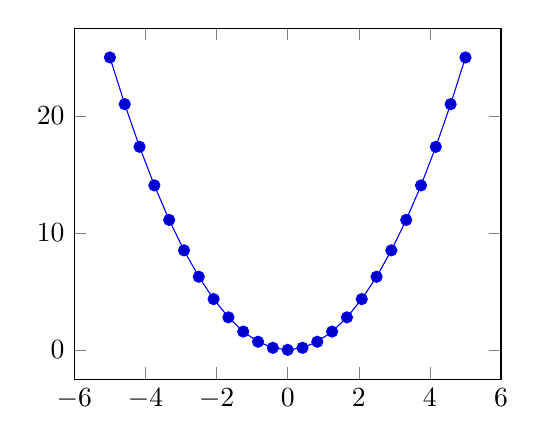
\begin{tikzpicture}
\begin{axis}
\addplot {x^2};
\end{axis}
\end{tikzpicture}
\caption{Our first external graphics example}
\end{figure}


\begin{figure}
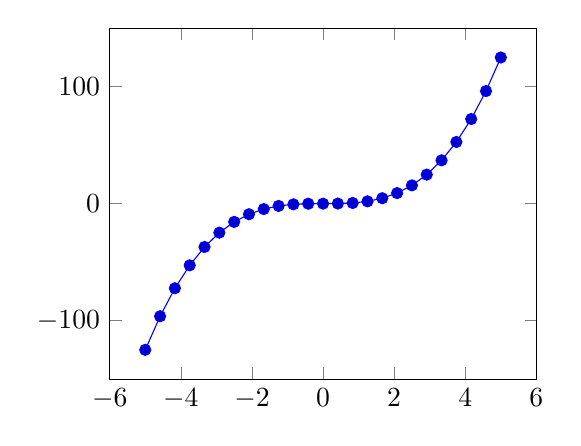
\begin{tikzpicture}
\begin{axis}
\addplot {x^3};
\end{axis}
\end{tikzpicture}
\caption{A second graphics}
\end{figure}




\tikzsetnextfilename{3Dplot}
\begin{figure}
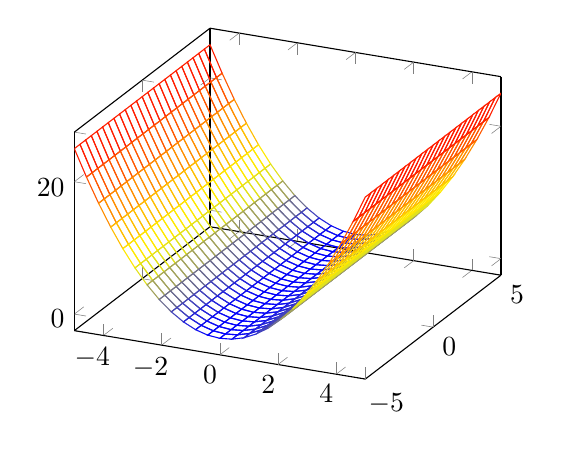
\begin{tikzpicture}
\begin{axis}
\addplot3[mesh] {x^2};
\end{axis}
\end{tikzpicture}
\caption{Our third external graphics example}
\end{figure}


\tikzsetnextfilename{Surfaceplot}
\begin{figure}
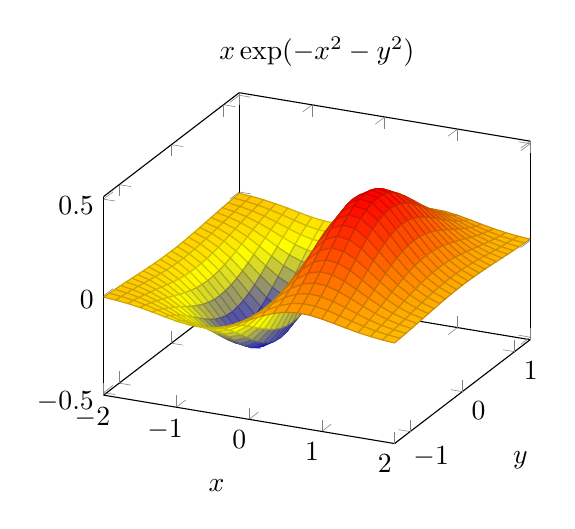
\begin{tikzpicture}
\begin{axis}[
title={$x \exp(-x^2-y^2)$},
xlabel=$x$, ylabel=$y$
]
\addplot3[
surf,
domain=-2:2,
domain y=-1.3:1.3,
]
{exp(-x^2-y^2)*x};
\end{axis}
\end{tikzpicture}
\caption{Our fourth external graphics example}
\end{figure}


\tikzsetnextfilename{normaldist}
\begin{figure}
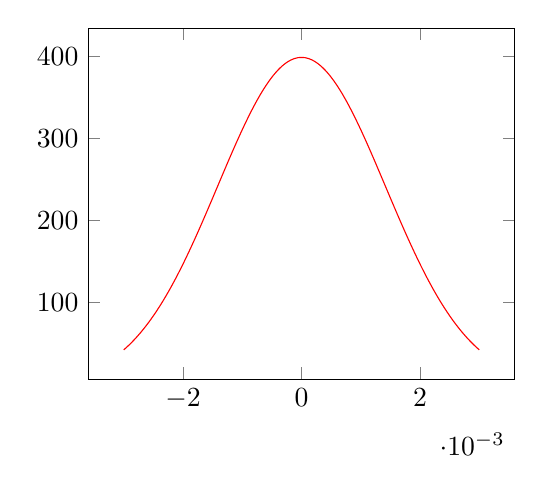
\begin{tikzpicture}
\begin{axis}[
]
% density of Normal distribution:
\addplot[
red,
domain=-3e-3:3e-3,
samples=201,
]
{exp(-x^2 / (2e-3^2)) / (1e-3 * sqrt(2*pi))};
\end{axis}
\end{tikzpicture}
\caption{Our fifth external graphics example}
\end{figure}



\chapter{Mathematical Notation} 


\begin{table}[ht]
	\centering
	\begin{tabular}{|l|l|l|}
		\hline
		Key & Rising factorial & $Q$\\
		\hline
		"m" & $(a_j)_m$ &  Yes \\
		"n" & $(a_j)_n$ &  Yes \\
		"m+n" & $(a_j)_{m+n}$ &  Yes \\				
		"m-n" & $(a_j)_{m-n}$ &  No \\
		"n-m" & $(a_j)_{n-m}$ &  No \\
		"2m+n" & $(a_j)_{2m+n}$ &  No \\				
		"2m-n" & $(a_j)_{2m-n}$ &  No \\
		"2n-m" & $(a_j)_{2n-m}$ &  No \\
		\hline
	\end{tabular}
%	\caption{\result}
%	\label{\result} 
\end{table}

{\bfseries\itshape\sffamily bold italic sans-serif type}

{\itshape\sffamily bold italic sans-serif type}

{\bfseries\sffamily bold italic sans-serif type}

{\sffamily bold italic sans-serif type}


$\begin{array}{lcl} z & = & a \\ f(x,y,z) & = & x + y + z \end{array}$

$
A_{m,n} =
\begin{pmatrix}
a_{1,1} & a_{1,2} & \cdots & a_{1,n} \\
a_{2,1} & a_{2,2} & \cdots & a_{2,n} \\
\vdots  & \vdots  & \ddots & \vdots  \\
a_{m,1} & a_{m,2} & \cdots & a_{m,n}
\end{pmatrix}
$


\begin{center}
	\begin{longtable}{p{4cm}  p{12cm}  }
		\caption{Notation related to Sets}\\
		%\hline
		%\noalign{\vskip 1.5mm}
		%\textbf{Item} & \textbf{Edition 2} \\
		%\noalign{\vskip 0.8mm}
		\hline
		\noalign{\vskip 1mm}
		\endfirsthead
		\multicolumn{2}{c}%
		{\tablename\ \thetable\ -- \textit{Continued from previous page}} \\
		\hline
		\noalign{\vskip 1.5mm}
		\textbf{Item} & \textbf{Edition 2}  \\
		\noalign{\vskip 0.8mm}
		\hline
		\noalign{\vskip 1mm}
		\endhead
		\hline \multicolumn{2}{r}{\textit{Continued on next page}} \\
		\endfoot
		\hline
		\endlastfoot
		$\mathbb{N}$ &	Set of natural numbers	\nomenclature{$\mathbb{N}$}{Set of natural numbers} \\
		$\mathbb{Z}$ &	Set of integer numbers	\nomenclature{$\mathbb{Z}$}{Set of integer numbers} \\
		$\mathbb{Q}$ &	Set of rational numbers	\nomenclature{$\mathbb{Q}$}{Set of rational numbers} \\
		$\mathbb{R}$ &	Set of real numbers	\nomenclature{$\mathbb{R}$}{Set of real numbers} \\
		$\mathbb{C}$ &	Set of complex numbers	\nomenclature{$\mathbb{C}$}{Set of complex numbers} \\
	\end{longtable}
\end{center}


\begin{center}
	\begin{longtable}{p{4cm}  p{12cm}  }
		\caption{General Notation}\\
		%\hline
		%\noalign{\vskip 1.5mm}
		%\textbf{Item} & \textbf{Edition 2} \\
		%\noalign{\vskip 0.8mm}
		\hline
		\noalign{\vskip 1mm}
		\endfirsthead
		\multicolumn{2}{c}%
		{\tablename\ \thetable\ -- \textit{Continued from previous page}} \\
		\hline
		\noalign{\vskip 1.5mm}
		\textbf{Item} & \textbf{Edition 2}  \\
		\noalign{\vskip 0.8mm}
		\hline
		\noalign{\vskip 1mm}
		\endhead
		\hline \multicolumn{2}{r}{\textit{Continued on next page}} \\
		\endfoot
		\hline
		\endlastfoot
		Required .Net Framework &	Cloudy with rain, across many northern regions. Clear spells across most of Scotland and Northern Ireland,
		but rain reaching the far northwest.	 \\
		Windows XP support for .NET & 	yes \\
		Support for .NET Charts &	no  \\
		Required .Net Framework &	2	 \\
		Windows XP support for .NET & 	yes \\
		Support for .NET Charts &	no  \\
		Required .Net Framework &	2	 \\
		Windows XP support for .NET & 	yes \\
		Support for .NET Charts &	no  \\
		Required .Net Framework &	2	 \\
		Windows XP support for .NET & 	yes \\
		Support for .NET Charts &	no  \\
		Required .Net Framework &	2	 \\
		Windows XP support for .NET & 	yes \\
		Support for .NET Charts &	no  \\
		Required .Net Framework &	2	 \\
		Windows XP support for .NET & 	yes \\
		Support for .NET Charts &	no  \\
		Required .Net Framework &	2	 \\
		Windows XP support for .NET & 	yes \\
		Support for .NET Charts &	no  \\
		Required .Net Framework &	2	 \\
		Windows XP support for .NET & 	yes \\
		Support for .NET Charts &	no  \\
		Required .Net Framework &	2	 \\
		Windows XP support for .NET & 	yes \\
		Support for .NET Charts &	no  \\
		Required .Net Framework &	2	 \\
		Windows XP support for .NET & 	yes \\
		Support for .NET Charts &	no  \\
	\end{longtable}
\end{center}




\end{document}
